%!TEX root =presentation.tex
\section[godunov]{Godunov discretization} % (fold)
\label{sec:godunov_discretization}

\subsection{Discretizing single system} % (fold)
\label{sub:discretizing_single_system}

% subsection discretizing_single_system (end)

\begin{frame}
\frametitle{Discretizing via Godunov method}

\begin{itemize}
    \item Cannot represent (or not practical to represent) continuous function on computer.
    \item Approximate solution by discretizing space and time.
    \item Solve for vector of discrete variables.
\end{itemize}

\begin{block}{Godunov's scheme (high level)}
\begin{enumerate}
    \item Split system in discrete chunks of size $\Delta x$.
    \item Approximate IC by averaging over $\Delta x$.
    \item Find exact sln of system by solving Riemann problems at discretized boundaries for $\Delta t$ time.
    \item Approximate new sln by averaging over $\Delta x$.
    \item Set IC as new sln and go to step 3.
\end{enumerate}
\end{block}

\end{frame}

\begin{frame}



\begin{figure}
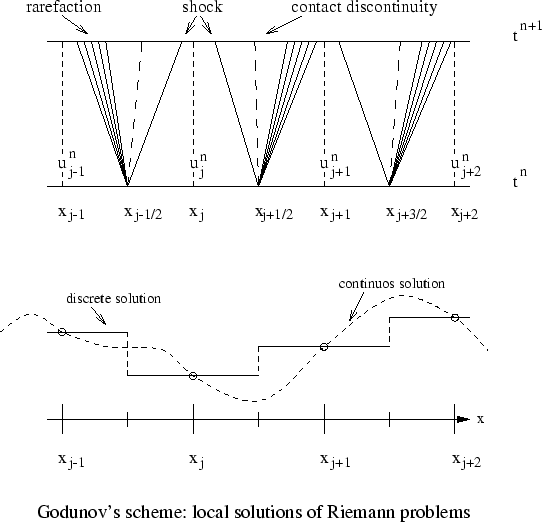
\includegraphics[width=.65\columnwidth]{images/godunov}
\caption{credit: http://www.uv.es/astrorela/simulacionnumerica/node34.html}
\end{figure}


\end{frame}

\begin{frame}
\frametitle{Derivation of Godunov's method}

Take discrete initial condition $\dvar_i$ at cell $i$. We want $\bar{\dvar})_i$, the average value at cell $i$ at time $\Delta t$:

\begin{equation}
    \bar{\dvar}_{i}=\dvar_{i}-\frac{1}{x_{i+1}-x_{i}}\int_{0}^{\Delta t}\left(f\left(u\left(t,x_{i+1}\right)\right)-f\left(u\left(t,x_{i}\right)\right)\right)dt
\end{equation}


This requires solution of $\cvar(x,t)$ over $[0,\Delta x]\times [0,\Delta t]$. 


But since Riemann problems are self-similar, fluxes across boundaries are constant:

\begin{equation}
    \int_{0}^{\Delta t}f\left(u\left(t,x_{i}\right)\right)dt\approx\Delta tg^{G}\left(\dvar_{i},\dvar_{i+1}\right)
\end{equation}

where $g^G$ is the flux across cell boundaries obtained via sln of Riemann problem.

Now only function of discrete values:

\begin{equation}
\bar{\dvar}_{i}=\dvar_{i}-\frac{\Delta t}{x_{i+1}-x_{i}}\left(g^{G}\left(\dvar_{i},\dvar_{i+1}\right)-g^{G}\left(\dvar_{i-1},\dvar_{i}\right)\right)    
\end{equation}


\end{frame}

\begin{frame}[t]\frametitle{CFL condition}

In previous derivation, it is assumed no solution from one Riemann problem influences another at the discrete boundaries.

This limits how large the time-step to guarantee convergence of Godunov scheme to continuous solution.

\begin{block}{The Courant Friedrichs Lewy (CFL) condition}
\begin{equation}
    \lambda^{\max}\le\frac{\Delta x}{\Delta t}
\end{equation}
\end{block}

\end{frame}

\subsection{Discretizing PDE network} % (fold)
\label{sub:discretizing_pde_network}

\begin{frame}

Solving for Godunov flux easy for $1$-to-$1$ junctions. What about $n$-to-$m$?

\begin{figure}
\includegraphics<1>[width=\columnwidth]{figs-gen/god-rp}
\includegraphics<2>[width=\columnwidth]{figs-gen/god-rp-sln}
\end{figure}

\begin{itemize}
    \item<2> Apply Riemann solver at junction
    \item<2> Use Riemann solution as boundary condition for $g^G$ at junction.
\end{itemize}

\end{frame}

\begin{frame}
\frametitle{Summary of Godunov scheme for PDE networks}


\begin{enumerate}
\item<1-> Begin with initial condition ($t=0$) $\left\{ \dvar_{\link}:\link\in\links\right\} $.
\item<2-> For every junction $\jn\in\jns$:
\begin{enumerate}
\item<2-> Apply the Riemann solver to Riemann data to obtain the boundary condition
$\hat{\mathbf{\dvar}}_{\jn}=\RS\left(\mathbf{\dvar}_{\jn}\right)$.
\end{enumerate}
\item<3-> For every link $\link\in\links$:

\begin{enumerate}
\item<3-> Letting $\jn_{\link}^{\text{Up}}=\jn\in\jns:\link\in Out\left(\jn\right)$
and $\jn_{\link}^{\text{Down}}=\jn\in\jns:\link\in In\left(\jn\right)$,
the discrete value over link $\link$ at time $\Delta t$, $\bar{\dvar}_{\link}$,
is given by:
\end{enumerate}

\[
\bar{\dvar}_{\link}=\dvar_{\link}-\frac{\Delta t}{L_{\link}}\left(f\left(\left\{ \mathbf{\hat{\dvar}}_{\jn_{\link}^{\text{Down}}}\right\} _{\link}\right)-f\left(\left\{ \mathbf{\hat{\dvar}}_{\jn_{\link}^{\text{Up}}}\right\} _{\link}\right)\right)
\]

\end{enumerate}

\begin{example}<4>
On board...
\end{example}

\end{frame}

% subsection discretizing_pde_network (end)

% section godunov_discretization (end)